%%% bpolynomial.tex
%%% Copyright 2007 Stephan Hennig <stephanhennig@arcor.de>
%
% This work may be distributed and/or modified under the conditions of
% the LaTeX Project Public License, either version 1.3 of this license
% or (at your option) any later version.  The latest version of this
% license is in http://www.latex-project.org/lppl.txt
%
\RequirePackage[resetfonts]{cmap}
\documentclass{article}
\usepackage[T1]{fontenc}
\usepackage{ae}
\usepackage{amsmath}
\usepackage{amssymb}
\newcommand*{\cmd}[1]{\texttt{#1}}
\newcommand*{\name}[1]{\textsf{#1}}
\newcommand*{\pkg}{\name{bpolynomial}}
\newcommand{\user}[1]{\emph{#1}}
\newcommand*{\B}{B\'ezier}
\usepackage{xcolor}
\colorlet{framecol}{black!50}
\usepackage{listings}
\lstloadlanguages{MetaPost,[LaTeX]TeX}
\lstset{language=MetaPost, basicstyle=\small\ttfamily, keywordstyle={}, commentstyle={}, columns=flexible, showspaces=false, showstringspaces=false, frame=single, rulecolor=\color{framecol}, aboveskip=2ex, belowskip=2ex, framesep=2ex, xleftmargin=2ex, xrightmargin=2ex}
\lstnewenvironment{listing}[1][]
{\lstset{#1}}
{}
\usepackage{multicol}
\usepackage{url}
\usepackage{graphicx}
\setcounter{topnumber}{1}
\setcounter{bottomnumber}{0}
\usepackage{ifpdf}
\ifpdf
\DeclareGraphicsRule{*}{mps}{*}{}
\fi

\begin{document}
\title{The \pkg\ package\thanks{This document describes \pkg\ v0.5, last revised 2007/12/12.}}
\author{Stephan Hennig\thanks{stephanhennig@arcor.de}}
\maketitle

\begin{abstract}
The MetaPost package \pkg\ helps plotting polynomial and root functions.  It provides macros to calculate one-segment \B\ curves exactly matching a given cubic polynomial or square or cubic root function.  Additionally, tangents on all functions and derivatives of polynomials can be calculated.
\end{abstract}

\setcounter{secnumdepth}{3}
\setcounter{tocdepth}{2}
\begin{multicols}{2}
\tableofcontents
\end{multicols}


\section{Introduction}\label{sec:intro}
MetaPost has a variable type \cmd{path} that can be used for drawing smooth and visualy pleasing curves.  When plotting graphs, the problem users are confronted with is how to define a suitable path representing a given function $f(x)$?

The \name{splines} package by Dan Luecking provides macros for drawing smooth piece-wise \B\ curves through arbitrary sample points of a function.~\cite{mp:splines}  Since \B\ curves are polynomials of degree three, for cubic polynomials we can do better and find a matching one-segment \B\ curve.  This package eases the task of finding a \B\ curve corresponding to a given function of the following types:
\begin{align}
f(x) & = ax^3 + bx^2 + cx + d \\
f(x) & = u \sqrt{x + v} + w \\
f(x) & = u \sqrt[3]{x + v} + w
\end{align}


\section{Usage}\label{sec:usage}
The \pkg\ package provides two flavours of user interfaces:
\begin{itemize}
\item  An advanced interface, that first requires a function to be defined and then provides access to the \B\ curve corresponding to the function, its tangent or derivative in a given intervall.
\item A plain interface, that gives instant access to the \B\ curve matching a given function in an intervall.
\end{itemize}
The plain interface is less powerful, but might be convenient in certain circumstances.  It is briefly described in section~\ref{sec:plaininterface}.  The average user most likely wants to use the advanced interface, so we will discuss that first.

\subsection{Plotting polynomials}\label{sec:polynomials}
\subsubsection{Defining polynomials}\label{sec:newBPolynomial}
As was said before, calculating the \B\ curve of a polynomial function first requires a function to be defined.  The macro for defining a polynomial
\begin{equation}
  f(x) = ax^3 + bx^2 + cx + d
\end{equation}
is called
\begin{center}
  \cmd{newBPolynomial}
\end{center}
and takes five arguments.  First argument is a suffix and the remaining four arguments are the four coefficients of the polynomial function $a$, $b$, $c$, $d$.

A definition of a polynomial
\begin{equation}
  f(x) = 2x^3 + 0x^2 - 3x - 1  
\end{equation}
associated with suffix \cmd{f} exemplary looks like this
\begin{listing}
newBPolynomial.f(2, 0, -3, -1);
\end{listing}

The suffix argument \cmd{f} serves as an identifier for deriving names of other macros, that are defined by \cmd{newBPolynomial}.  To be more precise, command
\begin{center}
  \cmd{newBPolynomial.<suffix>}
\end{center}
defines three new macros
\begin{center}
  \begin{tabular}{l}
    \cmd{<suffix>.getPath} \\
    \cmd{<suffix>.eval} \\
    \cmd{<suffix>.getTangent} \\
  \end{tabular}
\end{center}
that do the real work.  These macros are described in the following sections.

\subsubsection{Getting the \B\ curve of a polynomial}\label{sec:getPath}
Once a polynomial $\langle$suffix$\rangle$ is defined, the macro to request a \B\ curve matching the function on an intervall $[x_l, x_r]$ is
\begin{center}
  \cmd{<suffix>.getPath}
\end{center}
This macro takes two argument, the intervall boundaries $x_l$ and $x_r$, and returns a polynomial shaped \B\ curve corresponding to function $\langle$suffix$\rangle$.  Command \cmd{<suffix>.getPath} can be called as often as required with varying intervall boundaries and always returns a path corresponding to the new intervall.

Let's have a look at an example.  Plotting our polynomial $f(x)$ on the intervall $(-2, 2)$ can be done with the following code (figure~\ref{fig:cubic}).
\begin{listing}
  newBPolynomial.f(2, 0, -3, -1);
  draw f.getPath(-2, 2) transformed T;
\end{listing}

\begin{figure}
%   \begin{minipage}[t]{.45\linewidth}
    \centering
    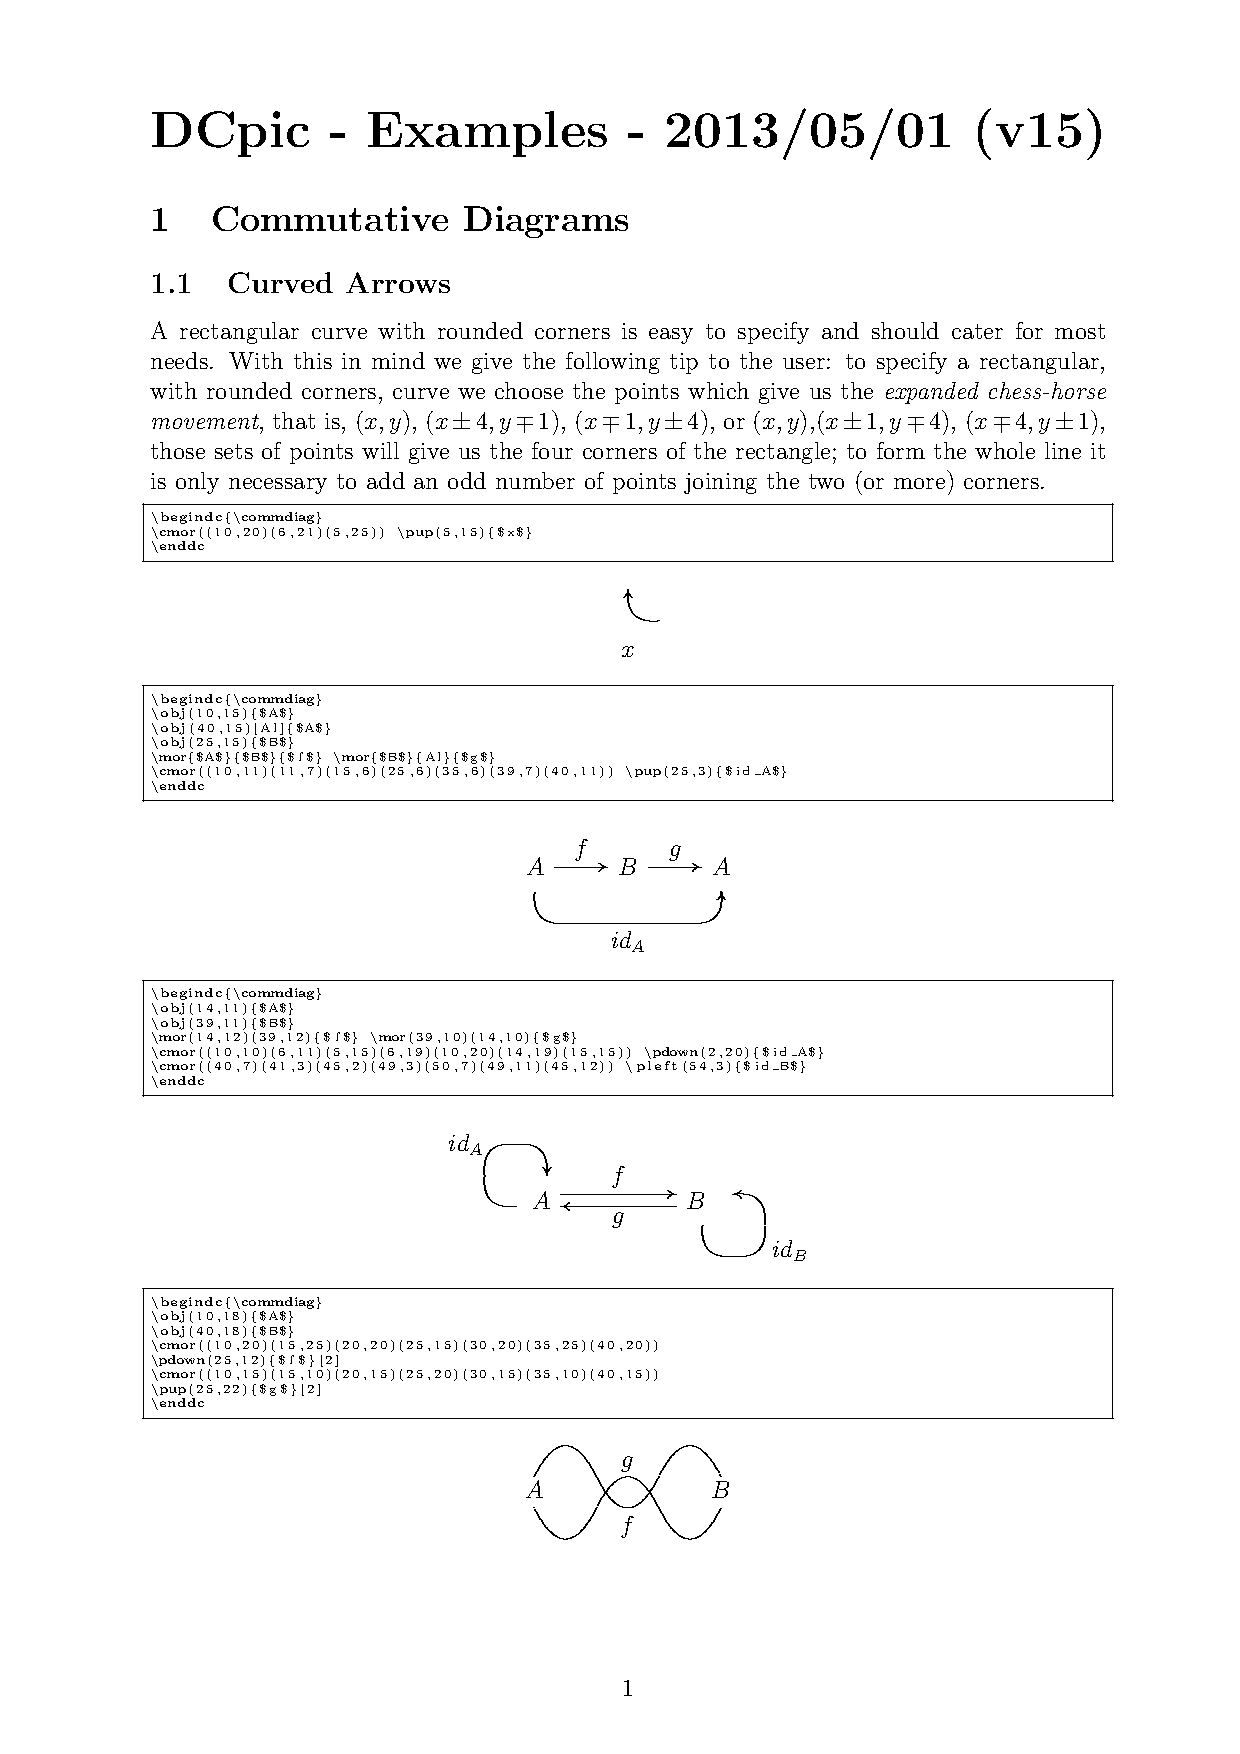
\includegraphics{examples.1}
    \caption{A cubic polynomial.}
    \label{fig:cubic}
%   \end{minipage}
\end{figure}

\emph{Hint:} Since the \pkg\ package never uses $\langle$suffix$\rangle$ as a complete identifier, you can use that as the name of a path variable to store the path returned by \cmd{<suffix>.getPath} for later drawing.  Any other path (array) variable serves the same purpose, though.
\begin{listing}
  newBPolynomial.f(2, 0, -3, -1);
  path f;
  f := f.getPath(-2, 2);
  draw f transformed T;
\end{listing}

Note, since the base unit of MetaPost is a big point ($1\,\text{bp}=\frac{1}{72}\,\text{in}$) in most cases functions have to be scaled to a proper size before plotting.  It is \emph{not} recommended, however, to apply scaling to polynomial coefficients, since current MetaPost versions can't handle large numbers very well.%
\footnote{At the time of writing the latest release is MetaPost v1.002.}
Instead, scaling should be applied to paths during \cmd{draw} operations.  If not stated otherwise, in this manual, scaling is applied by an affine transform
\begin{center}
  \cmd{T = identity xscaled 10mm yscaled 1mm;}
\end{center}

\subsubsection{Getting a tangent on a polynomial}\label{sec:getTangent}
Another macro set up during a function definition is
\begin{center}
  \cmd{<suffix>.getTangent}
\end{center}
This macro returns a path tangent to a function $\langle$suffix$\rangle$ at a specific point.  Arguments are an $x$-coordinate, where the tangent is placed, and two values $\epsilon_l$, $\epsilon_r$ that specify the neighbourhood around $x$.  The tangent path then covers the intervall $[x+\epsilon_l,x+\epsilon_r]$.  This syntax has been choosen to make it easy to move a tangent along a function, keeping its neighbourhood at a fixed size.

As an example, the following code draws a tangent that touches $f$ at $x=-0.5$ with a neighbourhood $\epsilon = \pm 1$ (figure~\ref{fig:tangent}).%
\footnote{Both types of arguments to \cmd{f.getTangent}---$x$ and $\epsilon$ values---have been put in separate pairs of parentheses to make the code more readable.  Even if the second pair of parentheses looks like a coordinate of type \cmd{pair}---it isn't.  For MetaPost this syntax is equivalent to
  \begin{center}
    \cmd{draw f.getTangent(-0.5, -1, 1) transformed T;}
  \end{center}
}
\begin{listing}
  newBPolynomial.f(2, 0, -3, -1);
  draw f.getPath(-2, 2) transformed T;
  draw f.getTangent(-0.5)(-1, 1) transformed T;
\end{listing}

\begin{figure}
  \begin{minipage}[t]{.45\linewidth}
    \centering
    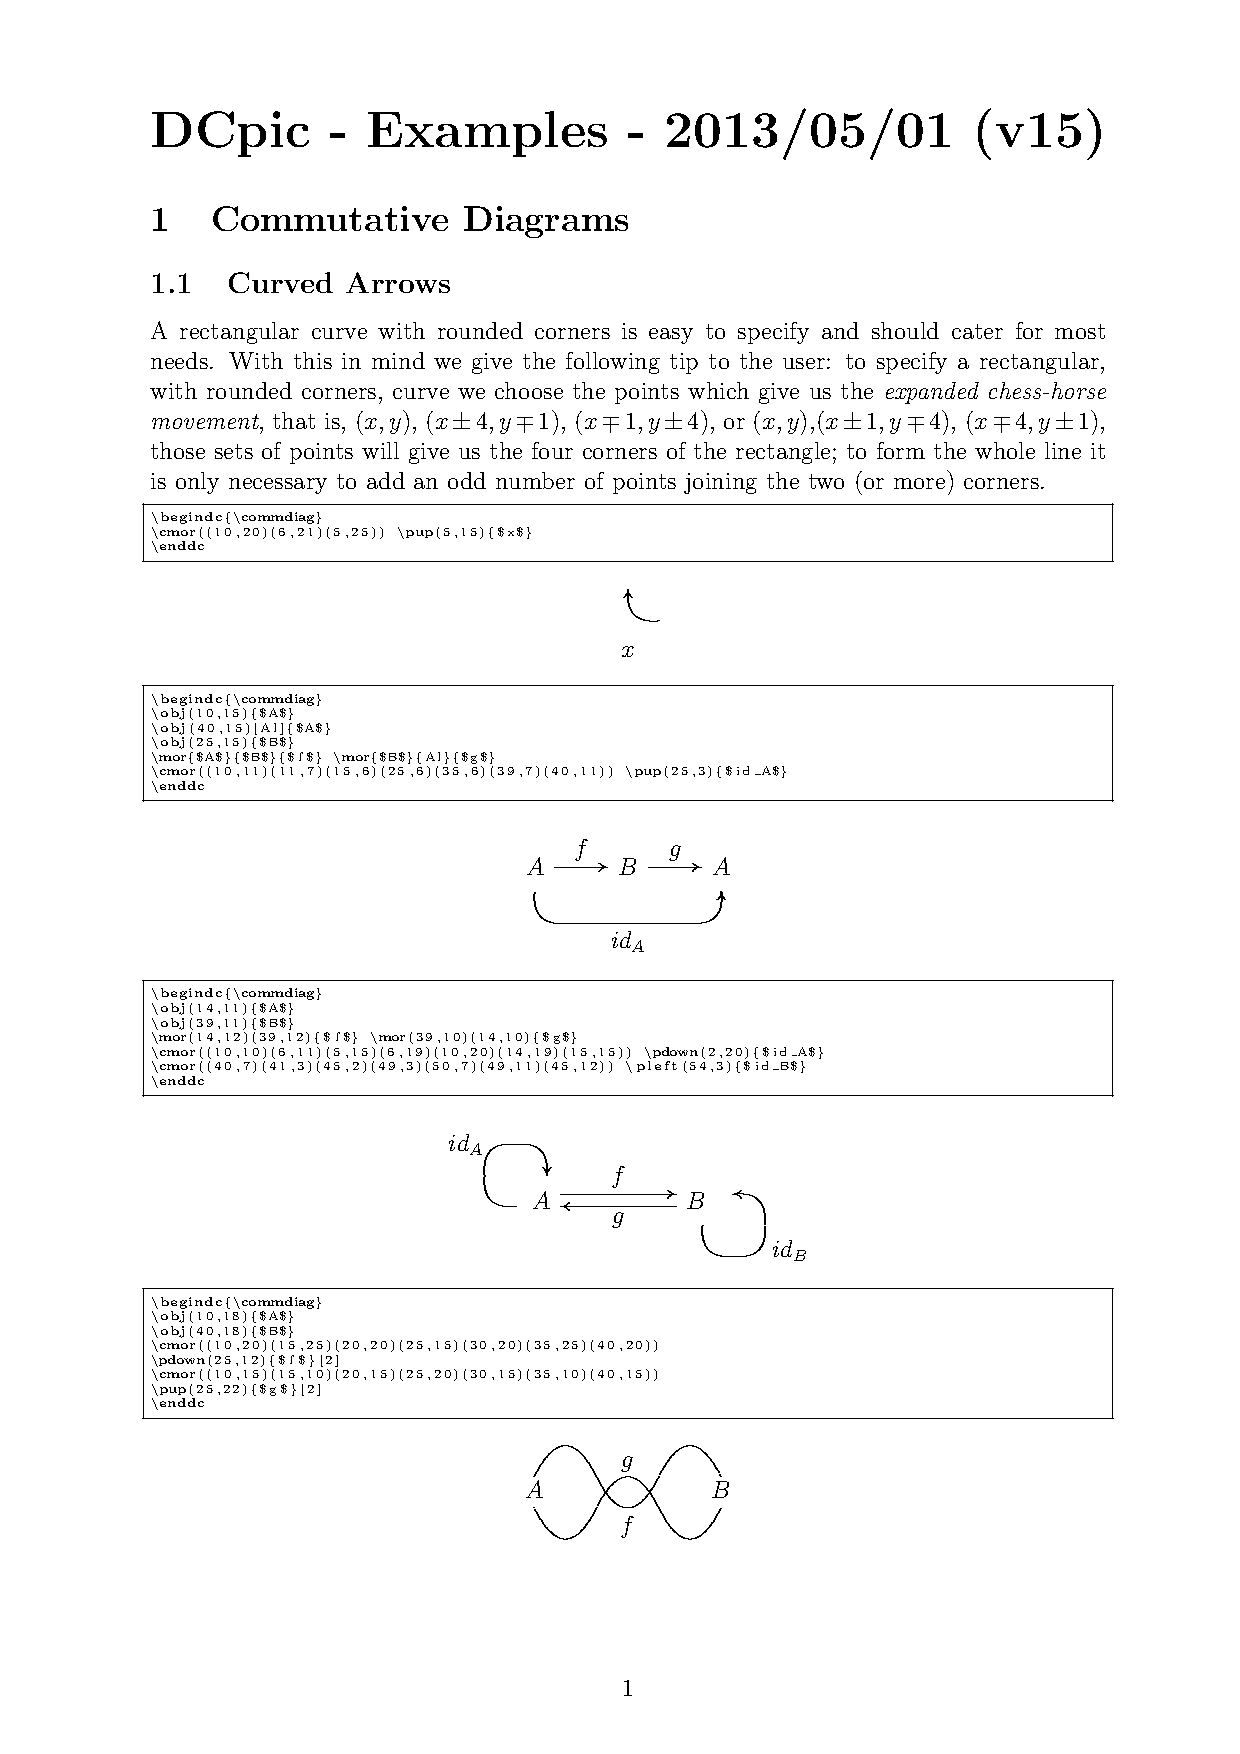
\includegraphics{examples.2}
    \caption{Cubic polynomial with a tangent.}
    \label{fig:tangent}
  \end{minipage}\hfill%
  \begin{minipage}[t]{.45\linewidth}
    \centering
    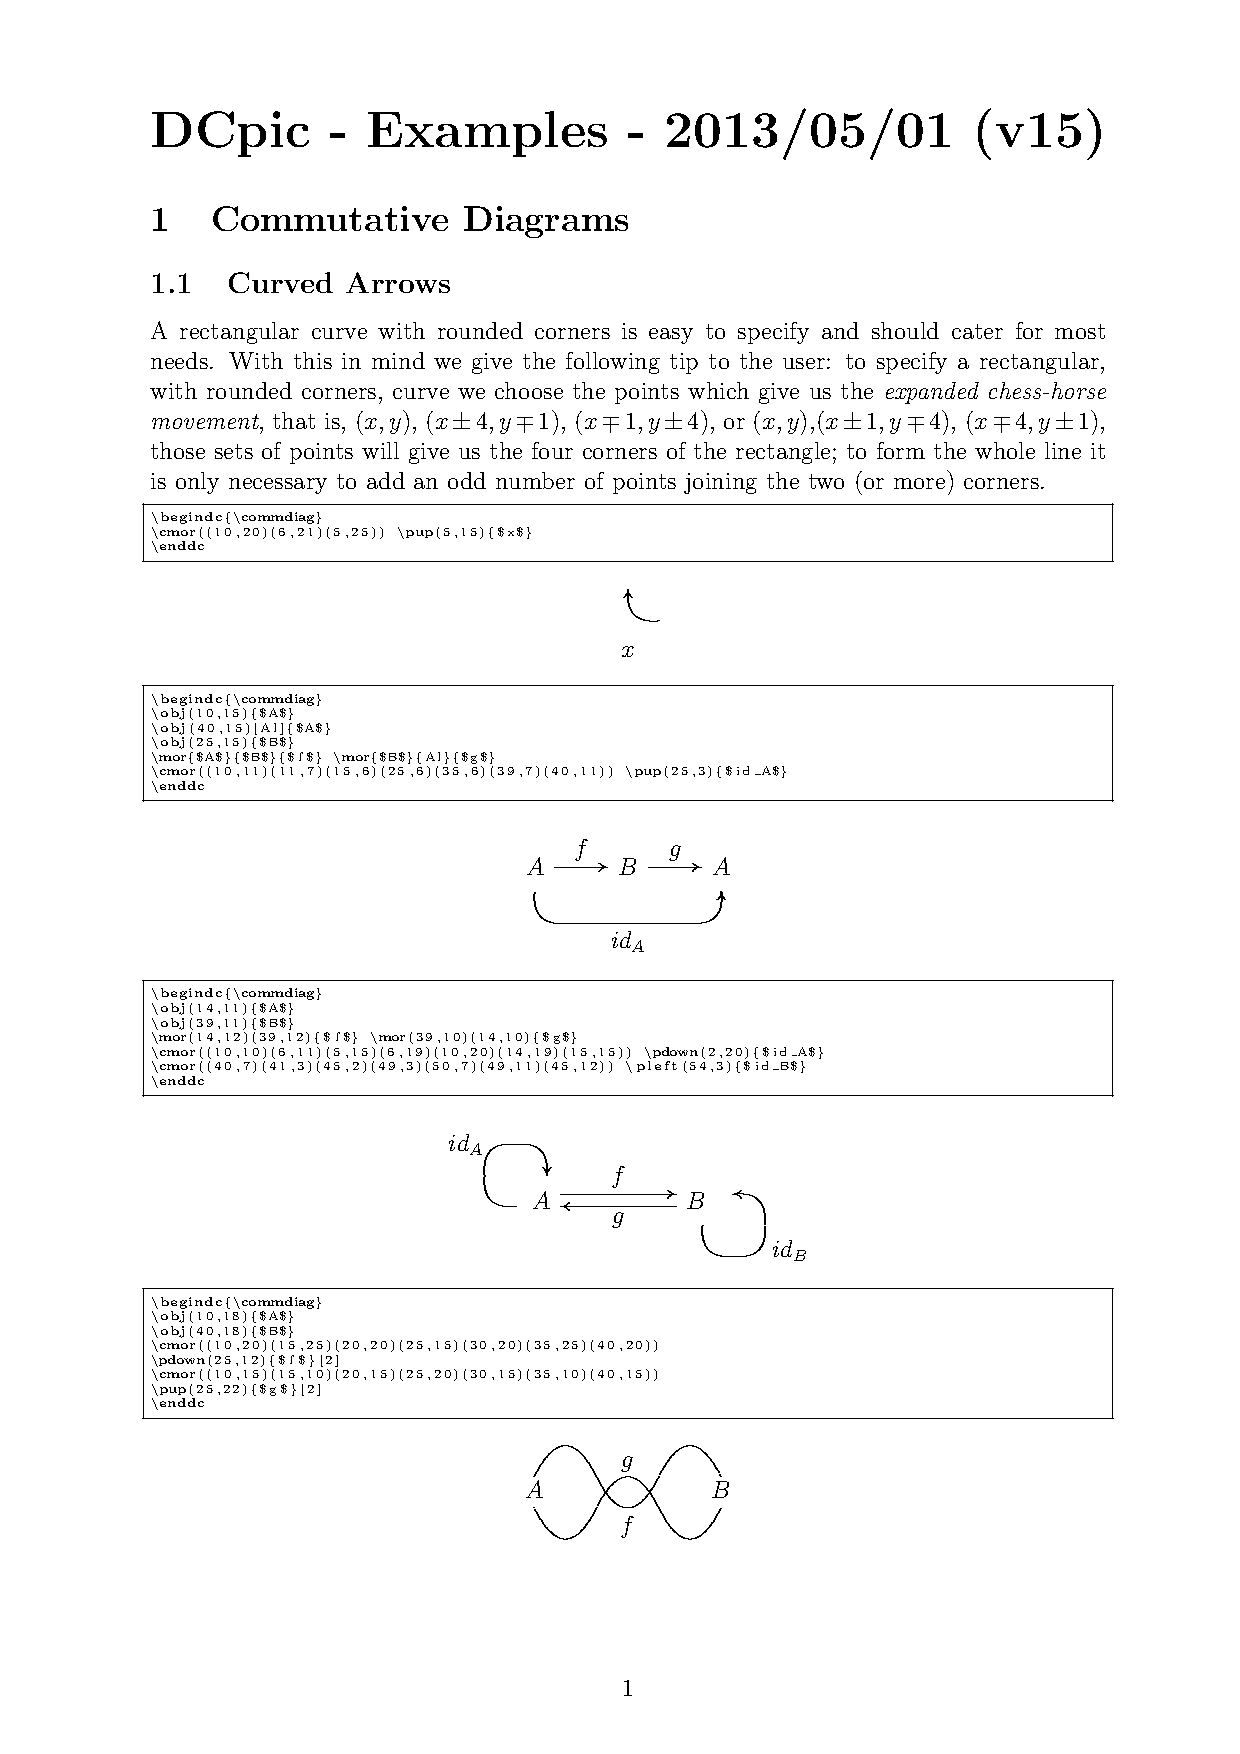
\includegraphics{examples.3}
    \caption{And a labelled point.}
    \label{fig:labelled}
  \end{minipage}
\end{figure}

\subsubsection{Evaluating polynomials}\label{sec:eval}
Additionally to getting the \B\ curve or tangent of a polynomial, polynomial functions can also be evaluated numerically at a specific location.  Defining a function $\langle$suffix$\rangle$ sets up a macro
\begin{center}
  \cmd{<suffix>.eval}
\end{center}
that takes as argument an $x$-coordinate and returns the function value at that location.  As an example, labelling an arbitrary point on $f$ can be done as follows (figure~\ref{fig:labelled}).
\begin{listing}
  dotlabeldiam := 2bp;
  labeloffset := 10bp;
  newBPolynomial.f(2, 0, -3, -1);
  draw f.getPath(-2, 2) transformed T;
  x := -0.5;
  show (x, f.eval(x));
  draw f.getTangent(x)(-1, 1) transformed T;
  dotlabel.top(btex $(-0.5, 0.25)$ etex, (x, f.eval(x)) transformed T);
\end{listing}

For simplicity, the label has been provided explicitly in this example (after reading the coordinates off the \cmd{log} file).  But it is also possible to attach the correct coordinates automatically with the help of the MetaPost package \name{LaTeXMP} and \LaTeX\ package \name{numprint}.  While the former helps passing dynamically generated text from MetaPost to \LaTeX, the latter can be used to format and round numbers.~\cite{latex:numprint, mp:latexmp}.

\subsection{Plotting square and cubic roots}\label{sec:roots}
Two other types of functions can be described by \B\ curves:  square and cubic roots%
\footnote{The reason square and cubic roots can be expressed in terms of \B\ curves is that both are inverse functions of cubic polynomials.  More information can be found in appendix~\ref{app:roots}.}%
.  The \pkg\ package provides support for square and cubic root functions of the following type
\begin{align}
  f_{sqr}(x) = u \sqrt{x + v} + w\label{eq:square} \\
  f_{cub}(x) = u \sqrt[3]{x + v} + w\label{eq:cubic}
\end{align}
through macros
\begin{center}
  \begin{tabular}{l}
    \cmd{newBSqrRoot} \\
    \cmd{newBCubRoot} \\
  \end{tabular}
\end{center}

These macros are similar to \cmd{newBPolynomial}.  Both macros take as arguments a suffix $\langle$suffix$\rangle$ and the three parameters $u$, $v$ and $w$ of the respective function.  They define three macros
\begin{center}
  \begin{tabular}{l}
    \cmd{<suffix>.getPath} \\
    \cmd{<suffix>.eval} \\
    \cmd{<suffix>.getTangent} \\
  \end{tabular}
\end{center}
that can be used the same way as for polynomial functions.

There is one notable difference between polynomial and root functions.  While polynomials $z^k$ are defined for all arguments $z \in \mathbb{R}$, roots $\sqrt[k]{z}$ are only defined for non-negative arguments $z \in \mathbb{R_+}$ and therefore the functions from equations~\ref{eq:square} and~\ref{eq:cubic} are only defined for
\begin{equation}
   x \geq -v.\label{eq:rootargument}
\end{equation}

In case the arguments to macros \cmd{<suffix>.getPath}, \cmd{<suffix>.getTangent} or \cmd{<suffix>.eval} violate equation~\ref{eq:rootargument} all macros write a warning to the log file, but go on with their calculations replacing the arguments in question (or the resulting range boundaries) by $-v$.

The following example plots two functions $s(x) = \sqrt{x}$ and $c(x) = \sqrt[3]{x}$ with a tangent on $s$ at $x=3$ (figure~\ref{fig:squareroot}).
\begin{listing}
  T := identity scaled 10mm;
  newBSqrRoot.s(1,0,0);
  newBCubRoot.c(1,0,0);
  draw s.getPath(0,6) transformed T;
  draw c.getPath(0,6) transformed T;
  draw s.getTangent(3)(-2, 2) transformed T;
\end{listing}

\begin{figure}
  \begin{minipage}[t]{.55\linewidth}
    \centering
    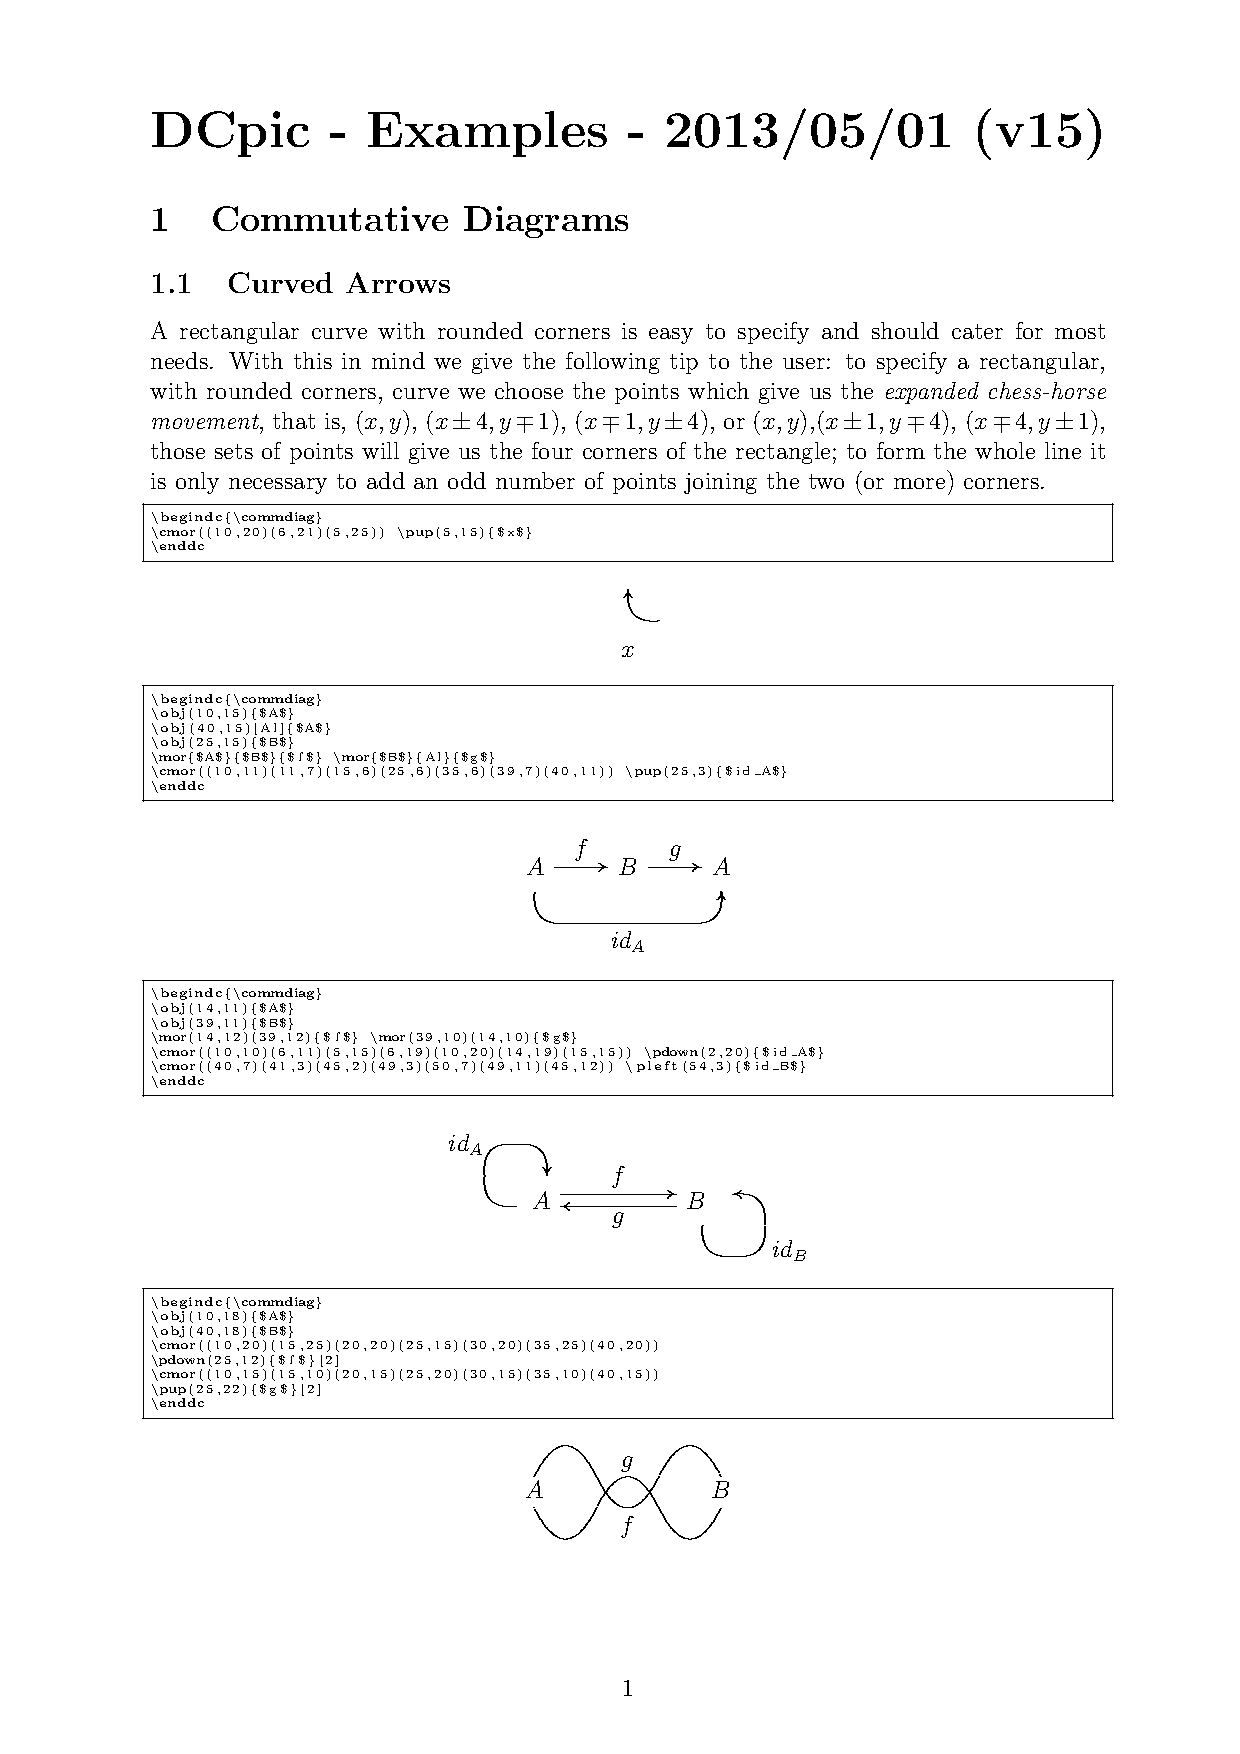
\includegraphics{examples.5}
    \caption{Square and cubic roots with a tangent.}
    \label{fig:squareroot}
  \end{minipage}\hfill%
  \begin{minipage}[t]{.4\linewidth}
    \centering
    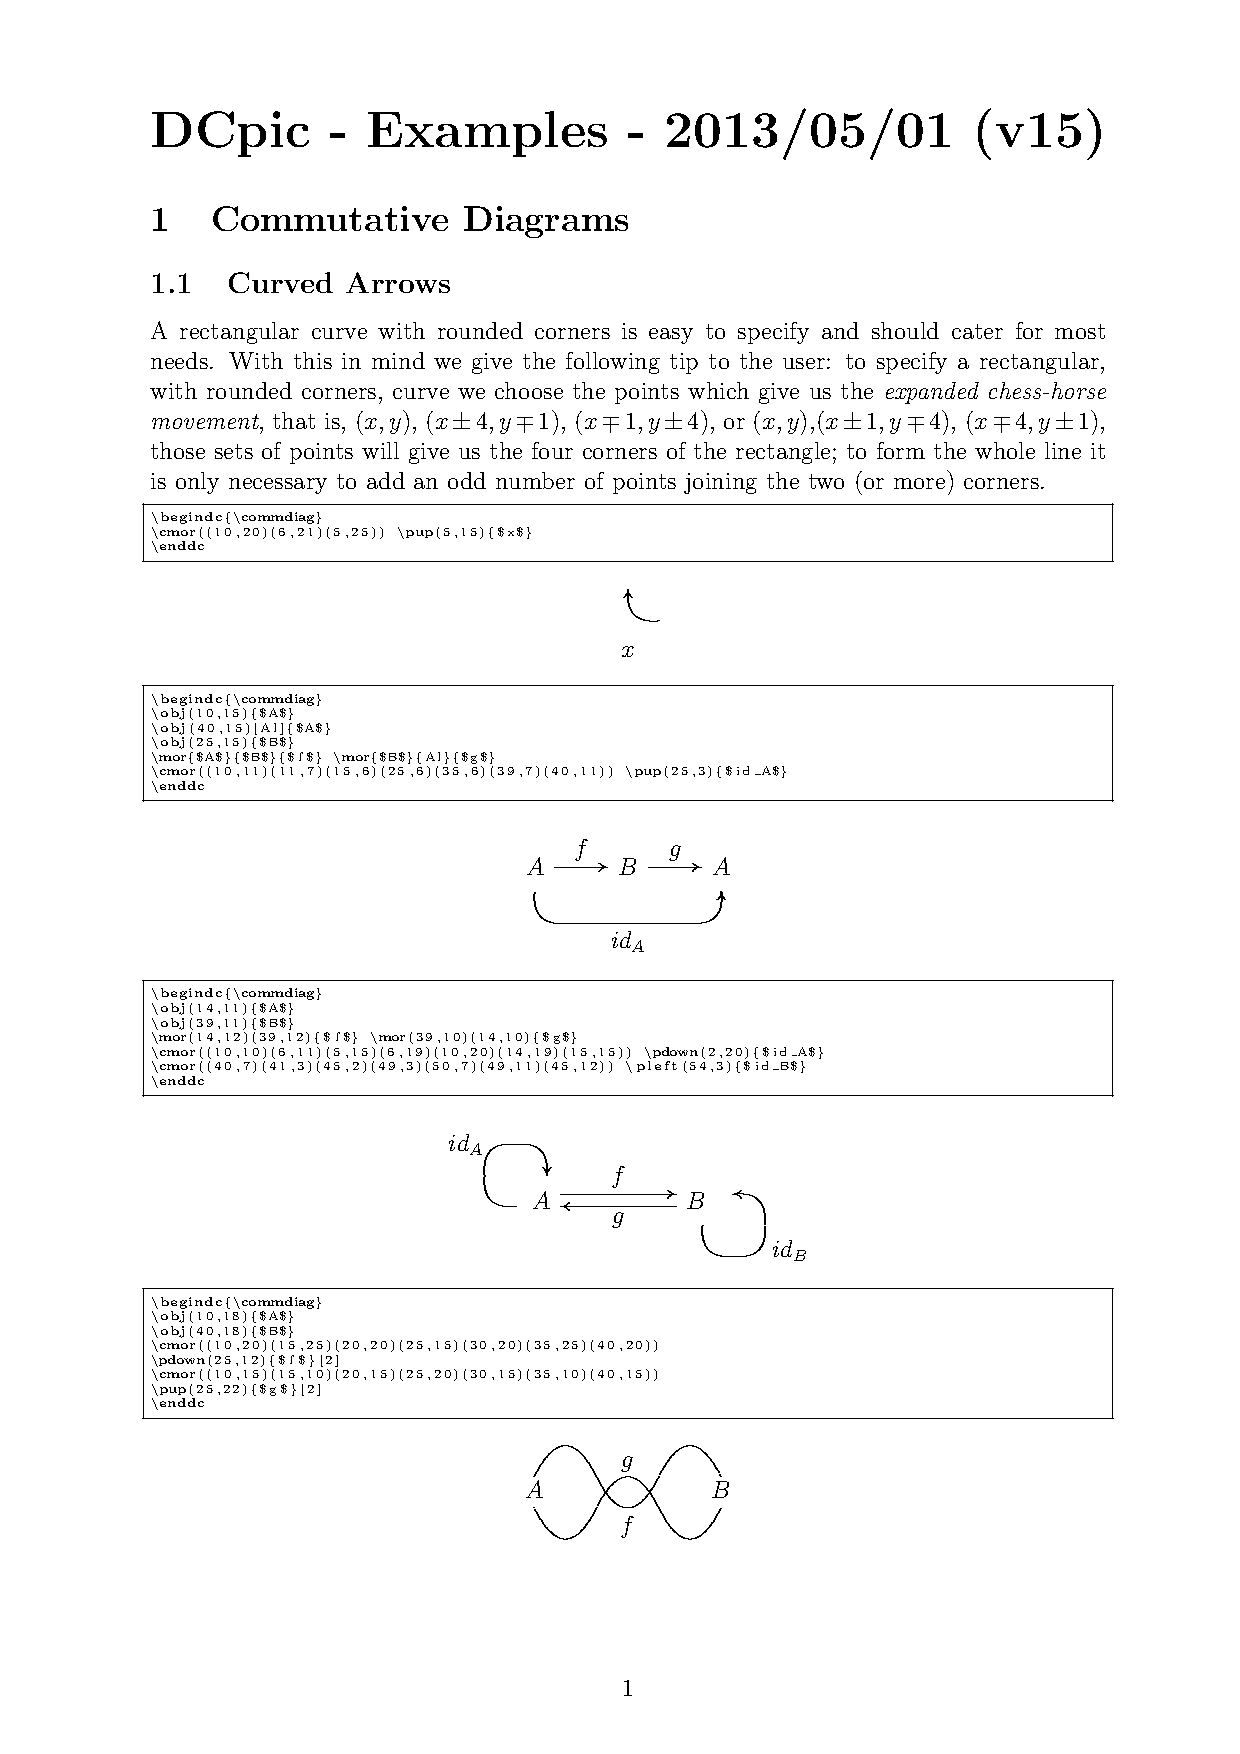
\includegraphics{examples.4}
    \caption{First derivative of a cubic polynomial with tangent.}
    \label{fig:derivative}
  \end{minipage}
\end{figure}

\subsection{Dealing with derivatives}\label{sec:derivatives}
Since plotting function often involves plotting derivatives of functions, too, the \pkg\ package provides support for plotting derivatives of polynomials and tangents thereof.  Unfortunately, derivatives of root functions cannot be described by \B\ curves, so those are not supported.

In section~\ref{sec:newBPolynomial} it was said macro \cmd{newBPolynomial} defines three new macros.  But this is not the full story.  In fact, the command
\begin{center}
  \cmd{newBPolynomial.<suffix>}
\end{center}
defines twelve macros, three of them we already know, \cmd{<suffix>.getPath}, \cmd{<suffix>.eval}, \cmd{<suffix>.getTangent}.  The remaining nine macros are similar, but correspond to the first, second and third derivative of a polynomial $\langle$suffix$\rangle$, resp.  To access these macros just add the required number of prime characters to the suffix name (three at maximum).  For instance, to get the path corresponding to the first derivative of polynomial $\langle$suffix$\rangle$ call
\begin{center}
  \cmd{<suffix>'.getPath}
\end{center}
and to get a tangent on the first derivative call
\begin{center}
  \cmd{<suffix>'.getTangent}.
\end{center}

In total these are the macros defined by \cmd{newBPolynomial.<suffix>}:
\begin{center}
  \begin{minipage}{.77\textwidth}
  \begin{multicols}{2}
    \cmd{<suffix>.getPath} \\
    \cmd{<suffix>.eval} \\
    \cmd{<suffix>.getTangent} \\
    \cmd{<suffix>'.getPath} \\
    \cmd{<suffix>'.eval} \\
    \cmd{<suffix>'.getTangent} \\
    \cmd{<suffix>'{}'.getPath} \\
    \cmd{<suffix>'{}'.eval} \\
    \cmd{<suffix>'{}'.getTangent} \\
    \cmd{<suffix>'{}'{}'.getPath} \\
    \cmd{<suffix>'{}'{}'.eval} \\
    \cmd{<suffix>'{}'{}'.getTangent}
  \end{multicols}
\end{minipage}
\end{center}

As an example, the following code draws a tangent on the first derivative of a polynomial \cmd{f} (figure~\ref{fig:derivative}).

\begin{listing}
  newBPolynomial.f(2, 0, -3, -1);
  draw f'.getPath(-2, 2) transformed T;
  draw f'.getTangent(-0.25)(-1, 1) transformed T;
\end{listing}


\subsection{Accessing function parameters}\label{sec:parameters}
The parameters passed to one of the function defining macros are saved for internal calculations.  These variables can be accessed by users, too, but should not be changed.

Defining a polynomial with
\begin{center}
  \cmd{newBPolynomial.<suffix>(<a>, <b>, <c>, <d>)}
\end{center}
defines variables
\begin{center}
  \begin{minipage}{.77\textwidth}
  \begin{multicols}{2}
    \cmd{<suffix>.a} \\
    \cmd{<suffix>.b} \\
    \cmd{<suffix>.c} \\
    \cmd{<suffix>.d} \\
    \cmd{<suffix>'.a} \\
    \cmd{<suffix>'.b} \\
    \cmd{<suffix>'.c} \\
    \cmd{<suffix>'.d} \\
    \cmd{<suffix>'{}'.a} \\
    \cmd{<suffix>'{}'.b} \\
    \cmd{<suffix>'{}'.c} \\
    \cmd{<suffix>'{}'.d} \\
    \cmd{<suffix>'{}'{}'.a} \\
    \cmd{<suffix>'{}'{}'.b} \\
    \cmd{<suffix>'{}'{}'.c} \\
    \cmd{<suffix>'{}'{}'.d}
  \end{multicols}
\end{minipage}
\end{center}
and sets them to the value of the corresponding coefficient.

For root functions the following variables are used:
\begin{center}
  \begin{tabular}{l}
    \cmd{<suffix>.u} \\
    \cmd{<suffix>.v} \\
    \cmd{<suffix>.w} \\
  \end{tabular}
\end{center}

Additionally, variables
\begin{center}
  \begin{tabular}{l}
    \cmd{<suffix>.a} \\
    \cmd{<suffix>.b} \\
    \cmd{<suffix>.c} \\
    \cmd{<suffix>.d} \\
  \end{tabular}
\end{center}
contain the coefficients of the inverse polynomial function.

\subsection{The plain interface}\label{sec:plaininterface}
The \pkg\ package provides a plain interface, too.  This interface avoids the necessity to define a function prior to calculating paths, but is limited to calculating \B\ curves of explicitly given polynomials and root functions---tangents and derivatives are not supported.  The plain interface consists of three macros
\begin{center}
  \begin{tabular}{l}
    \cmd{getBezierFromPolynomial} \\
    \cmd{getBezierFromSqrRoot} \\
    \cmd{getBezierFromCubRoot} \\
  \end{tabular}
\end{center}
that take as arguments the parameters of the polynomial or root function plus the range the path should cover.

For instance, the first example could as well have been drawn with the following code
\begin{listing}
  draw getBezierFromPolynomial(2, 0, -3, -1)(-2, 2) transformed T;
\end{listing}

All three macros call a macro \verb+bpolynomial_getBezierFromPolynomial+ behind the scenes, that does the necessary calculations and, in fact, is the heart of this package.  The mathematics behind that macro are described in appendix~\ref{app:mathematics}.


\section{Examples}\label{sec:examples}
This section contains some more elaborate examples.  The code of all examples is copied here, so that you can easily compare it with the resulting figures.  If you want to play around with the code you can also find it in file \cmd{examples.mp}, that actually contains the code of all examples in this manual.

\emph{One additional note in advance:}  While playing with figure~\ref{fig:transparency}, the author noticed a subtle rendering bug in Adobe Reader~7.0.9, that caused the graphs and the filled area not matching exactly.  In print or with GSview~4.8 and Ghostscript~8.60 everything looked fine.  The problem is actually unrelated to the filling, but there seem to be some numeric issues in the \B\ curve rendering algorithm of Adobe Reader.  A work-around is to modifiy problematic paths, \emph{e.\,g.}, by slightly changing their plotting range.

The first example demonstrates how \pkg\ and John Hobby's \name{graph} package\cite{mp:graph} can be used together to plot polynomials in a coordinate system.  The \cmd{draw} command has just to be replaced by \cmd{gdraw}.  The latter command additionally clips paths to the boundaries of the coordinate system (see figure~\ref{fig:graph.mp}).  Finally, in this example a table of points is printed to the console and \cmd{log} file.

\begin{figure}
  \centering
  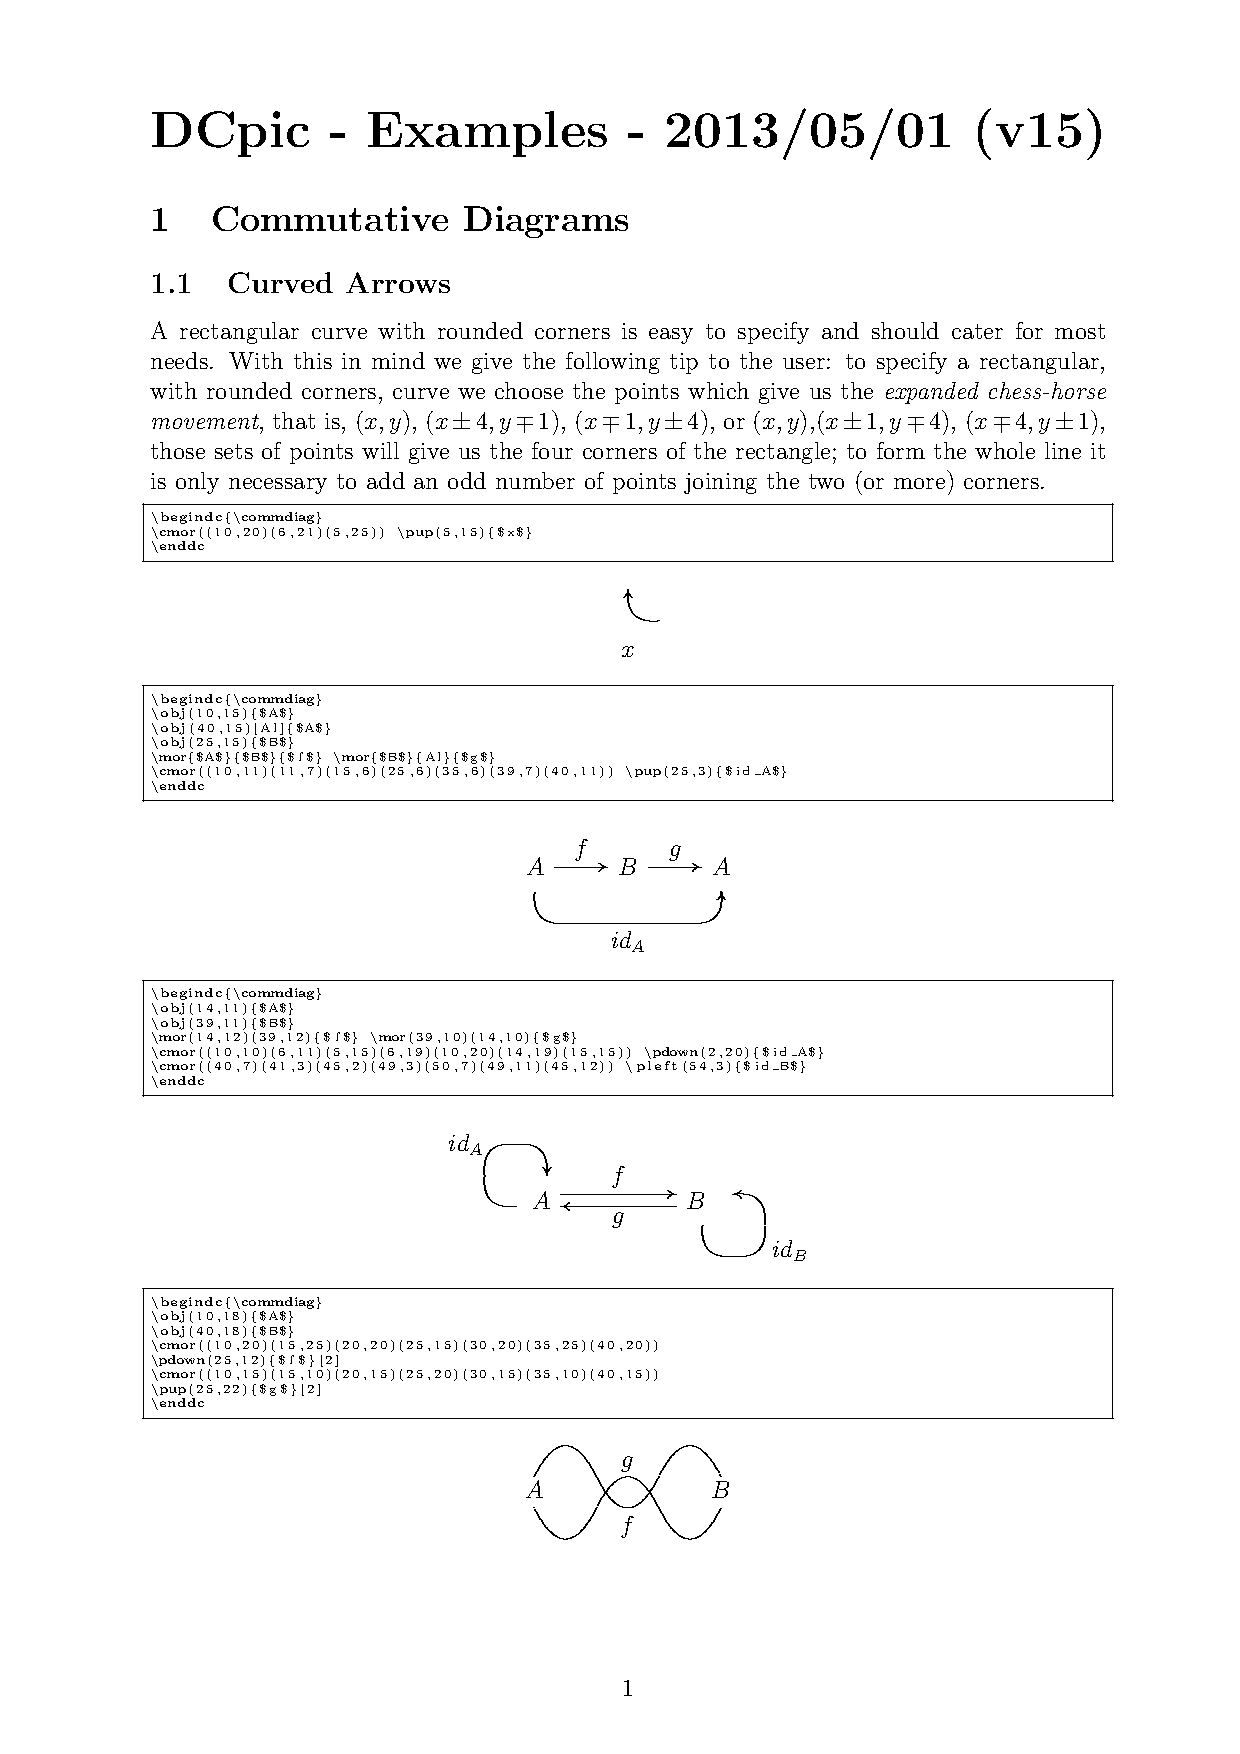
\includegraphics{examples.21}
  \caption{Packages \pkg\ and \name{graph} interacting.}
  \label{fig:graph.mp}
\end{figure}

\begin{listing}
path f, g;
  xmin := -7; xmax := 7;
  ymin := -7; ymax := 7;
  %%% Define polynomials f and g.
  newBPolynomial.f(0.3, 0, -3, -1);
  f := f.getPath(xmin, xmax);
  newBPolynomial.g(0, 0.5, -2, 0);
  g := g.getPath(xmin, xmax);
  %%% Draw graph.
  draw begingraph(10cm, 6cm);
    setrange(xmin,ymin, xmax,ymax);
    autogrid(grid.bot, grid.lft) dashed evenly withcolor .9white;
    drawoptions(withpen pencircle scaled 1bp);
    gdraw f;
    gdraw g dashed evenly scaled 2;
    drawoptions();
  endgraph;
  show f;
  %%% Write table with some points of f to log file.
  show "Polynomial: " & decimal f.a & "x^3 + " &
    decimal f.b & "x^2 + " & decimal f.c & "x + " & decimal f.d;
  for x=-5 upto 5:
    show (x, f.eval(x));
  endfor
\end{listing}

Note command \cmd{show f} that writes path~\cmd{f} to the \cmd{log} file.  Inspecting that we can easily verify \cmd{f} consists of just one path segment:
\begingroup\small
\begin{verbatim}
(-7,-82.90105)..controls (-2.33333,108.90105) and (2.33333,-110.90105)
 ..(7,80.90105)
\end{verbatim}
\endgroup

In the next example, a cubic polynomial $f$ is plotted together with its derivatives $f'$, $f''$ and $f'''$.  Additionally, for all four functions the tangents are drawn at $x=2$.  Admittedly, the plot is a little bit crowded.  But it should only serve as an example (figure~\ref{fig:derivatives}).

\begin{figure}
  \centering
  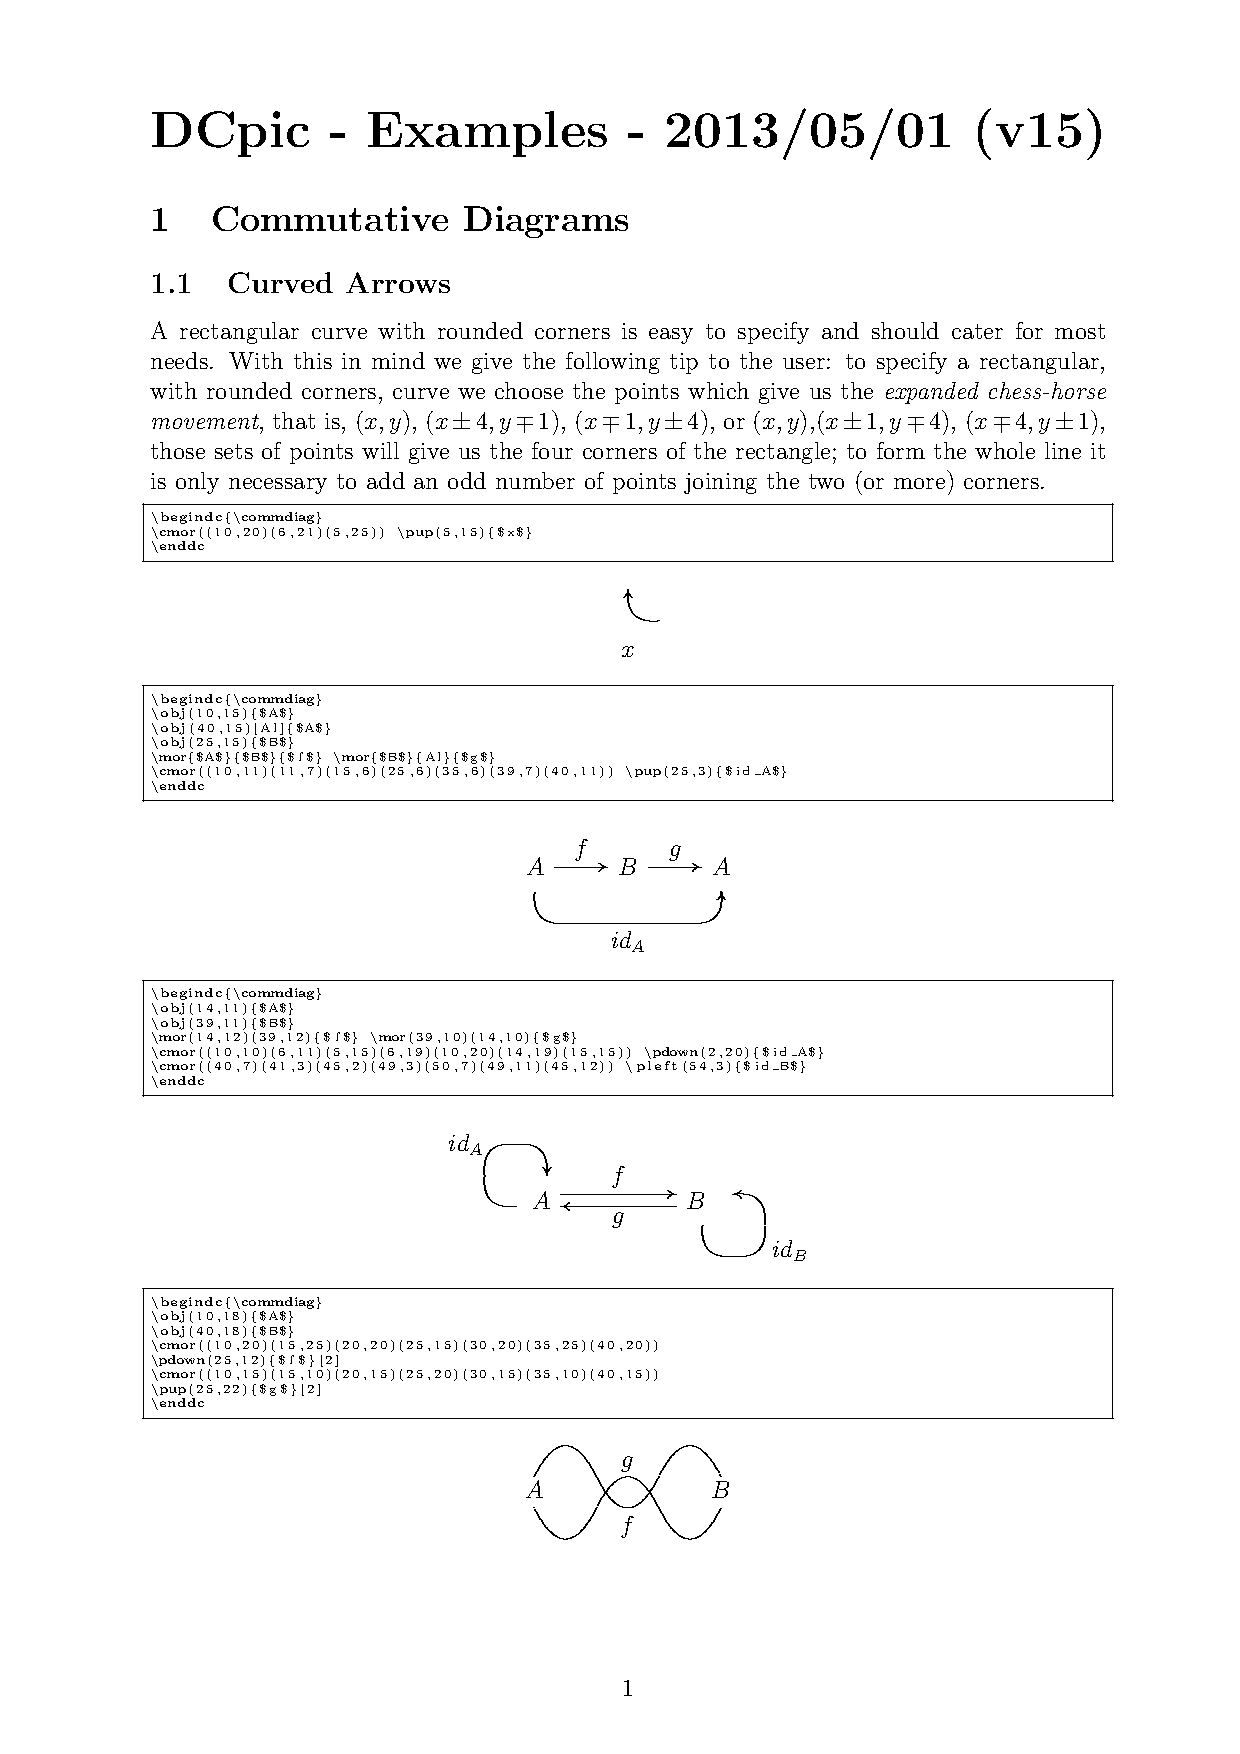
\includegraphics{examples.22}
  \caption{A cubic polynomial with derivatives and tangents.}
  \label{fig:derivatives}
\end{figure}

\begin{listing}
  xmin := -6; xmax := 6;
  ymin := -6; ymax := 6;
  newBPolynomial.f(0.3, -0.5, -0.5, -1);
  draw begingraph(10cm, 6cm);
    setrange(xmin,ymin, xmax,ymax);
    autogrid(grid.bot, grid.lft) dashed evenly withcolor .9white;
    drawoptions(withpen pencircle scaled 1bp);
    %%% Draw f and its derivatives f', f'', f'''.
    gdraw f.getPath(xmin, xmax);
    gdraw f'.getPath(xmin, xmax) dashed evenly scaled 2;
    gdraw f''.getPath(xmin, xmax) dashed withdots
      withpen pencircle scaled 2bp;
    gdraw f'''.getPath(-5, 5) withcolor .6white;
    %%% Draw tangents and mark points.
    x := 2;
    drawoptions(withcolor (1, 0.6, 0.6));
    gdraw f.getTangent(x)(-2, 2);
    gdraw f'.getTangent(x)(-1, 1);
    gdraw f''.getTangent(x)(-2, 2);
    gdraw f'''.getTangent(x)(-2, 2);
    drawoptions(withcolor (0.6, 0.6, 1));
    dotlabeldiam := 2.5bp;
    gdotlabel("", (x, f.eval(x)));
    gdotlabel("", (x, f'.eval(x)));
    gdotlabel("", (x, f''.eval(x)));
    gdotlabel("", (x, f'''.eval(x)));
    drawoptions();
  endgraph;
\end{listing}

How about some eye candy, \emph{e.\,g.}, transparency effects?  In the next example the area enclosed by two functions is filled with a transparent colour (figure~\ref{fig:transparency}).

Note, advanced PDF features like transparency and shadings are provided by package \name{metafun}.~\cite{mp:metafun}  Figures using such features have to be converted to stand-alone PDF files with the \cmd{mptopdf} utility before including them into a \LaTeX\ document.

\begin{figure}
    \centering
    \includegraphics{examples-23}
    \caption{Applying a transparent fill to an area enclosed by two functions.}
    \label{fig:transparency}
\end{figure}

\begin{listing}
path f, g, A;
  xmin := -3; xmax := 6;
  ymin := -3; ymax := 6;
  newBPolynomial.f(-0.25, 0.5, 2, -1);
  newBPolynomial.g(0, 0.5, -2, 0);
  f := f.getPath(-2.5, 5.5);
  g := g.getPath(-1.5, 5.5);
  %%% Find area between f and g.
  A := buildcycle(g, reverse f);
  draw begingraph(10cm, 6cm);
    setrange(xmin,ymin, xmax,ymax);
    autogrid(grid.bot, grid.lft) dashed evenly withcolor .9white;
    %%% Fill area with transparent colour.
    gfill A withcolor transparent (1, .3, (1, 0.5, 0));
    drawoptions(withpen pencircle scaled 1bp);
    gdraw f;
    gdraw g dashed evenly scaled 2;
    drawoptions();
  endgraph;
\end{listing}

As an alternative to solid fills areas can be emphasized by hatch patterns.  Hatching support is provided by package \name{hatching}.~\cite{mp:hatching}  Unfortunately, packages \name{graph} and \name{hatching} do not work together.  Therefore, in the next example a simple coordinate system had to be drawn manually (figure~\ref{fig:hatching.mp}).

\begin{figure}
  \centering
  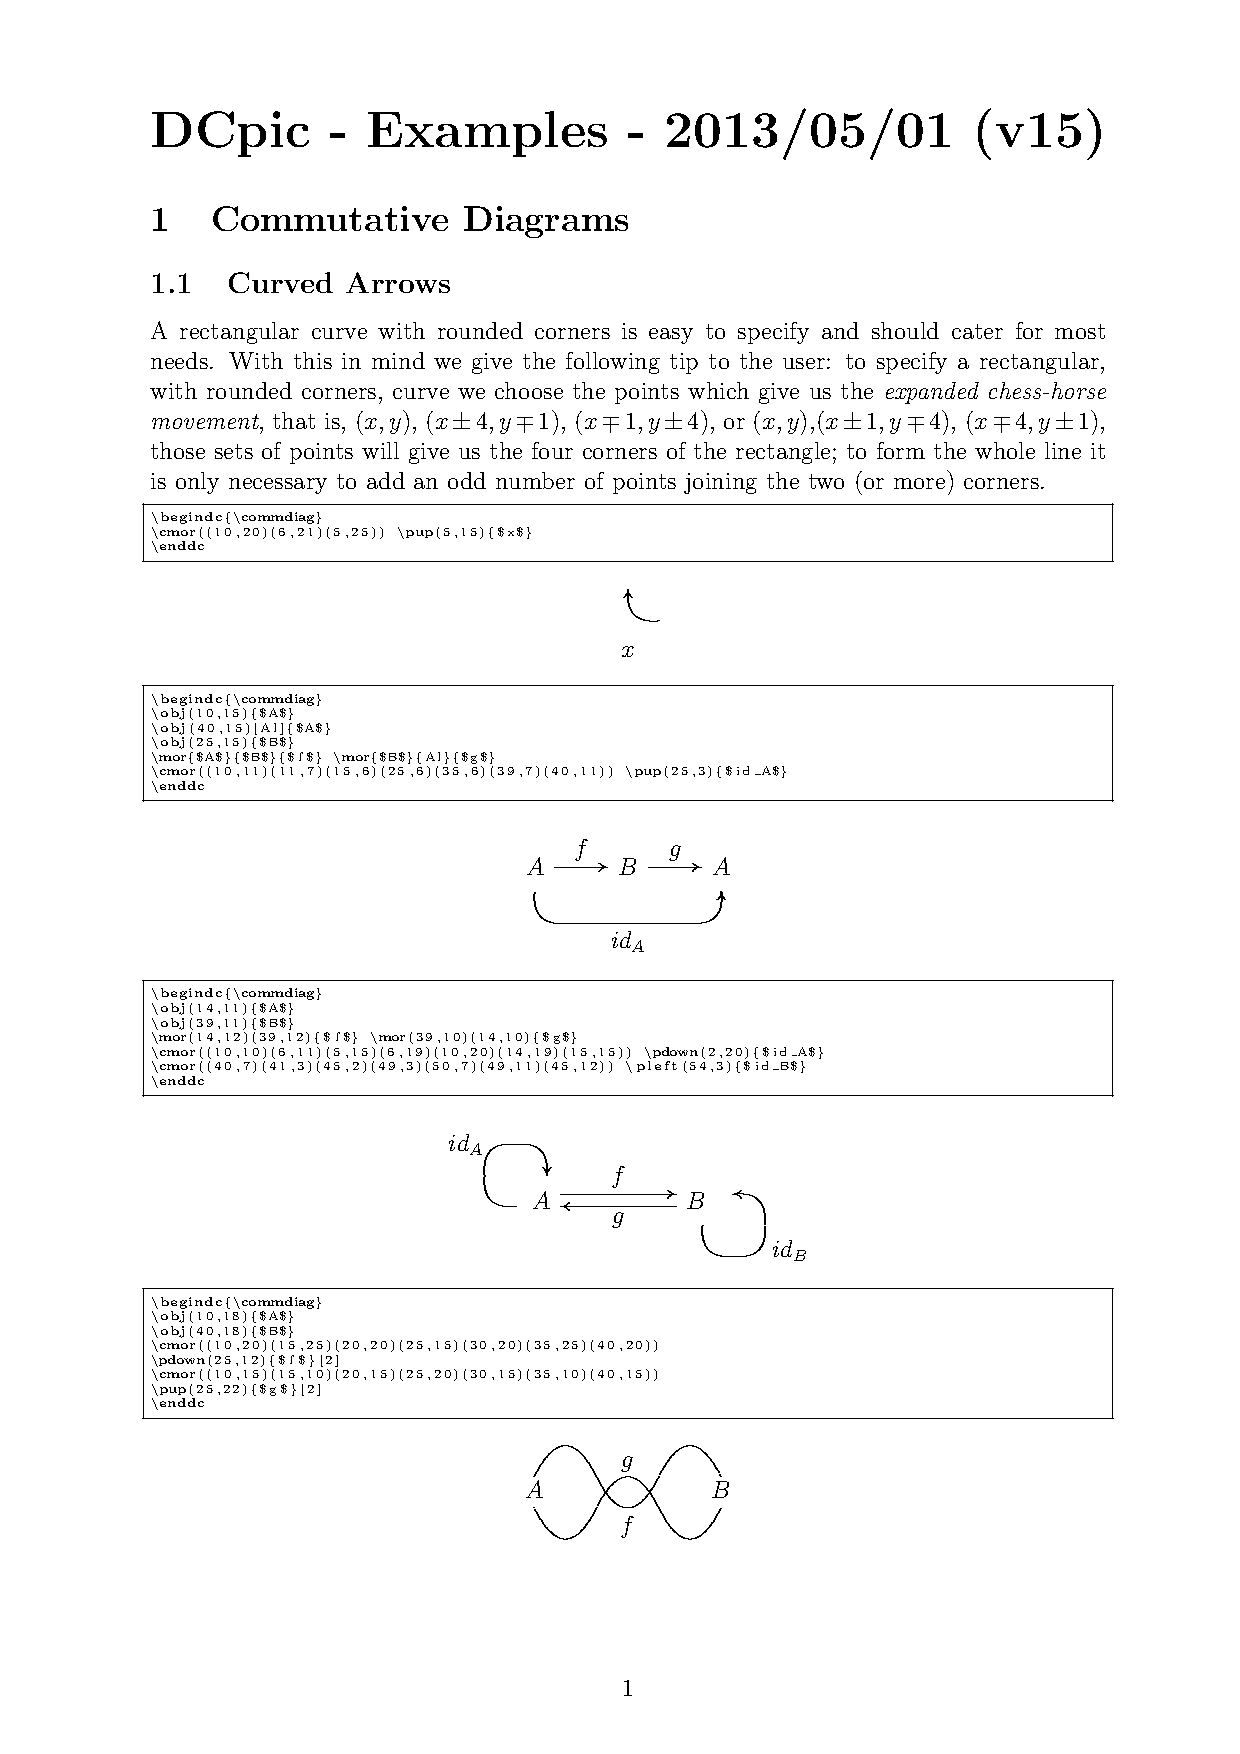
\includegraphics{examples.14}
  \caption{Hatching an area enclosed by two functions.}
  \label{fig:hatching.mp}
\end{figure}

\begin{listing}
path f, g, A;
  T := identity xscaled 10mm yscaled 6mm;
  %%% Draw coordinate system.
  xmin := -3; xmax := 6;
  ymin := -3; ymax := 6;
  drawoptions(withpen pencircle scaled 1bp withcolor 0.8white);
  drawarrow ((xmin,0)--(xmax,0)) transformed T;
  drawarrow ((0,ymin)--(0,ymax)) transformed T;
  newBPolynomial.f(-0.25, 0.5, 2, -1);
  newBPolynomial.g(0, 0.5, -2, 0);
  f := f.getPath(-2.5, 4.2);
  g := g.getPath(-1, 5);
  A := buildcycle(g, reverse f);
  %%% Fill area with pattern.
  drawoptions();
  hatchoptions(withcolor (0.6, 0.3, 0.3));
  hatchfill A transformed T
    withcolor (-45, 2mm, -0.5bp) withcolor (45, 2mm, -0.5bp);
  drawoptions(withpen pencircle scaled 1bp);
  draw f transformed T;
  draw g transformed T dashed evenly scaled 2;
\end{listing}


\appendix
\section{Calculating \B\ curves}\label{app:mathematics}
\subsection{Polynomials}\label{app:polynomials}
%Internally, paths are \B\ curves and MetaPost is able to calculate the points along such a curve.%
%\footnote{Since PostScript has a concept of \B\ curves, too, for MetaPost drawing a path is simply an act of copying the parameters of the corresponding \B\ curve into PostScript output.  But nonetheless MetaPost \emph{can} calculate points on a \B\ curve.}
%
A \B\ curve $P(t)$ with end points $A=(x_A,y_A)$ and $D=(x_D,y_D)$ and control points $B=(x_B,y_B)$ and $C=(x_C,y_C)$ is defined as~\cite{mfbook}
\begin{equation}
P(t) = \left(
  \begin{array}{@{}c@{}}
    x\\
    y\\
  \end{array}
  \right)(t) = (1-t)^3A + 3(1-t)^2tB + 3(1-t)t^2C + t^3D,\quad 0\leq t\leq 1.
\end{equation}

This equation can be rewritten as
\begin{equation}
P(t)  = A + 3(B-A)t + 3(C-2B+A)t^2 + (D-3C+3B-A)t^3,\quad 0\leq t\leq 1.
\end{equation}

An arbitrary function $y=f(x)$ can be written in parameter form as
\begin{equation}
  F(t) = \left(
    \begin{array}{@{}c@{}}
      x \\
      y \\
    \end{array}
  \right)(t) = \left(
    \begin{array}{@{}c@{}}
      x(t) \\
      f\big(x(t)\big) \\
    \end{array}
  \right),\quad t\in \mathbb{R}
\end{equation}
with parameter $t$.

For a polynomial function
\begin{equation}
  f(x) = ax^3 + bx^2 + cx + d,\quad x\in [x_0, x_1]
\end{equation}
we have
\begin{equation}
  x(t) = x_0 + (x_1-x_0)t,\quad 0\leq t\leq 1
\end{equation}
and hence
\begin{equation}
  F(t) = \left(
    \begin{array}{@{}c@{}}
      x_0 + (x_1-x_0)t \\
      ax(t)^3 + bx(t)^2 + cx(t) + d \\
    \end{array}
  \right),\quad 0\leq t\leq 1.
\end{equation}
Writing F(t) down explicitly is left as an exercise for the interested reader.

Finally, setting
\begin{equation}
  P(t) = F(t)
\end{equation}
and sorting the coefficients of the $t^k$ one arrives at the following \emph{original} equation system:
\begin{align}
  x_A & = x_0 \label{eq:xA} \\
  3(x_B-x_A) & = x_1 - x_0 \label{eq:xB} \\
  3(x_C-2x_B+x_A) & = 0 \label{eq:xC} \\
  x_D-3x_C+3x_B-x_A & = 0 \label{eq:xD} \\
  y_A & = ax_0^3 + bx_0^2 + cx_0 + d \label{eq:yA} \\
  3(y_B-y_A) & = 3ax_0^2(x_1-x_0) + 2bx_0(x_1-x_0) + c(x_1-x_0) \label{eq:yB} \\
  3(y_C-2y_B+y_A) & = 3ax_0(x_1-x_0)^2 + b(x_1-x_0)^2 \label{eq:yC} \\
  y_D-3y_C+3y_B-y_A & = a(x_1-x_0)^3 \label{eq:yD}
\end{align}
Note, there are only constants on the right-hand side of all equations.  That is, this equation system is linear in the eight variables $x_A$, $x_B$, $x_C$, $x_D$, $y_A$, $y_B$, $y_C$, $y_D$.

Since MetaPost can solve linear equation systems, hacking equations~\ref{eq:xA} to~\ref{eq:yD} into MetaPost code and requesting a path segment
\begin{center}\ttfamily
  ($x_A$,$y_A$)..controls ($x_B$,$y_B$) and ($x_C$,$y_C$)..($x_D$,$y_D$)
\end{center}
returns the polynomial shaped curve we are looking for.

Internally, the \pkg\ package does not solve the original equation system, but a \emph{modified} variant, that is numerically slightly more robust.

Equations~\ref{eq:xA} to~\ref{eq:xD} can be written down explicitly as
\begin{align}
  x_A & = x_0 \label{eq:xA'} \\
  x_B & = x_0 + \frac{1}{3}(x_1-x_0) \label{eq:xB'} \\
  x_C & = x_1 - \frac{1}{3}(x_1-x_0) \label{eq:xC'} \\
  x_D & = x_1 \label{eq:xD'}
\end{align}

Additionally, we know that $D=(x_D,y_D)$ is a point on the polynomial.  Therefore, equation~\ref{eq:yD} of the original system can be replaced by
\begin{align}
  y_D & = ax_1^3 + bx_1^2 + cx_1 + d \label{eq:yD'}
\end{align}

Equations~\ref{eq:yA} to~\ref{eq:yC} of the original equation system and the new equations~\ref{eq:xA'} to~\ref{eq:yD'} constitute the modified equation system, that is solved in \pkg.

\subsection{Square and cubic roots}\label{app:roots}
When requesting the \B\ curve of a root function, the \pkg\ package first calculates the inverse function, then calculates the corresponding path and finally reflects that on the function $f(x)=x$ to get the inverse again.

The inverse functions of the root functions from equations~\ref{eq:square} and~\ref{eq:cubic} are
\begin{align}
  \widetilde f_{sqr}(y) & = \left(\frac{y-w}{u}\right)^2 - v = 0 y^3 + \frac{1}{u^2} y^2 + \frac{-2w}{u^2} y + \frac{w^2}{u^2} - v \\
  \widetilde f_{cub}(y) & = \left(\frac{y-w}{u}\right)^3 - v = \frac{1}{u^3} y^3 + \frac{-3w}{u^3} y^2 + \frac{3w^2}{u^3} y + \frac{w^3}{u^3} - v
\end{align}
which both are clearly polynomials.

\nobreak
\bigskip
\raggedright
\parbox{\linewidth}{\itshape
  Happy \TeX ing!\par
  Stephan Hennig
}


\begin{thebibliography}{999}
\bibitem{mp:metafun} \textsc{Hagen}, Hans, \emph{metafun}, \url{http://www.pragma-ade.com/general/manuals/metafun-p.pdf}
\bibitem{latex:numprint} \textsc{Harders}, Harald, \emph{The numprint package}, 2007, \url{CTAN:macros/latex/contrib/numprint/numprint.pdf}
\bibitem{mp:graph} \textsc{Hobby}, John~D., \emph{Drawing graphs with MetaPost}, \url{http://www.tug.org/docs/metapost/mpgraph.pdf}
\bibitem{mp:hatching} \textsc{Jackowski}, B., \emph{hatching.mp}, \url{CTAN:graphics/metapost/contrib/macros/hatching/README}
\bibitem{mfbook} \textsc{Knuth}, Donald~E., \emph{The METAFONTbook}, Addison-Wesley, Reading, Massachusetts, 1986, (Computers \& Typesetting, C)
\bibitem{mp:splines} \textsc{Luecking}, Dan, \emph{Macros to compute splines}, 2005, \url{CTAN:graphics/metapost/contrib/macros/splines/splines.pdf}
\bibitem{mp:latexmp} \textsc{Morawski}, Jens-Uwe, \emph{latexMP}, 2005, \url{CTAN:graphics/metapost/contrib/macros/latexmp/doc/latexmp.pdf}
\end{thebibliography}

\end{document}

%%% Local Variables: 
%%% mode: latex
%%% TeX-PDF-mode: t
%%% TeX-master: t
%%% End: 
